\pdfminorversion=4
\documentclass[aspectratio=169,11pt]{beamer}
\usetheme{Madrid}
\usecolortheme{dolphin}
\setbeamertemplate{navigation symbols}{}
\setbeamertemplate{footline}{%
  \leavevmode\hbox{%
    \begin{beamercolorbox}[wd=.89\paperwidth,ht=2.9ex,dp=1.4ex,leftskip=1.3em]{author in head/foot}%
      \raisebox{-.45ex}{
\includegraphics[height=3.0ex]{figs/logo_ufci_rj_oficial.png}}%
      \hspace{.65em}{\scriptsize\bfseries UFCI/RJ}\hspace{.35em}{\scriptsize\textbar{} Ciência da Computação}%
    \end{beamercolorbox}%
    \begin{beamercolorbox}[wd=.11\paperwidth,ht=2.9ex,dp=1.4ex,rightskip=1.3em plus1fil]{date in head/foot}%
      \hfill\scriptsize\insertframenumber%
    \end{beamercolorbox}%
  }\vskip0pt%
}
\usepackage[T1]{fontenc}
\usepackage[utf8]{inputenc}
\usepackage[brazil]{babel}
\usepackage{lmodern}
\usepackage{amsmath,amssymb,booktabs,graphicx,multicol,array}
\usepackage{tikz}
\usetikzlibrary{arrows.meta,positioning,shapes.geometric,calc,fit}
\usepackage{listings}
\usepackage{xcolor}
\definecolor{azul}{HTML}{153653}
\definecolor{teal}{HTML}{137C87}
\definecolor{laranja}{HTML}{DA7F2B}
\definecolor{claro}{HTML}{EAF2F6}
\setbeamercolor{structure}{fg=azul}
\setbeamercolor{frametitle}{fg=white,bg=azul}
\setbeamercolor{block title}{fg=white,bg=azul}
\setbeamercolor{block body}{bg=blue!4}
\setbeamercolor{alerted text}{fg=teal}
\setbeamercolor{example text}{fg=teal}
\setbeamertemplate{itemize items}[circle]
\setlength{\parskip}{3pt}
\lstdefinestyle{prog}{language=C, basicstyle=\ttfamily\scriptsize,keywordstyle=\color{azul}\bfseries,commentstyle=\color{teal},stringstyle=\color{laranja!70!black},numbers=none,showstringspaces=false,columns=fullflexible,keepspaces=true,breaklines=true,frame=single,rulecolor=\color{blue!25},backgroundcolor=\color{blue!2},xleftmargin=3pt,framexleftmargin=3pt,aboveskip=2pt,belowskip=2pt}
\lstdefinestyle{terminal}{basicstyle=\ttfamily\footnotesize,keywordstyle=\color{teal},showstringspaces=false,columns=fullflexible,keepspaces=true,breaklines=true,frame=single,rulecolor=\color{blue!20},backgroundcolor=\color{blue!2},xleftmargin=4pt,framexleftmargin=4pt}
\title[Multiprocessamento e GPUs]{Arquitetura Avançada de Computadores}
\subtitle{Multiprocessamento e GPUs: primeiro programa CUDA na NVIDIA H100}
\author{Prof. Frederico Luís Cabral}
\institute{\textbf{UFCI/RJ} \textbar{} Ciência da Computação\\[1mm]\small Universidade Federal de Ciência e Inovação do Rio de Janeiro}
\date{}
\newcommand{\ideia}[1]{\begin{block}{Ideia central}#1\end{block}}
\newcommand{\pergunta}[1]{\begin{alertblock}{Para discutir}#1\end{alertblock}}
\begin{document}

% 01 - Capa institucional (logo oficial enviada pela UFCI/RJ)
\begin{frame}[plain]
\begin{tikzpicture}[remember picture,overlay]
  \fill[azul] (current page.north west) rectangle ([yshift=-.545\paperheight]current page.north east);
  \fill[teal] ([yshift=-.545\paperheight]current page.north west) rectangle ([yshift=-.557\paperheight]current page.north east);
\end{tikzpicture}
\vspace*{.45cm}
\begin{columns}[c,onlytextwidth]
\begin{column}{.69\textwidth}
{\color{white}\LARGE\bfseries Arquitetura Avançada\par de Computadores}\par
\vspace{.35cm}
{\color{white}\large Multiprocessamento e GPUs}\par
\vspace{.12cm}
{\color{white}\normalsize Primeiro programa CUDA na NVIDIA H100}
\end{column}
\begin{column}{.28\textwidth}
\centering
\begin{tikzpicture}
  \node[fill=white,rounded corners=5pt,inner sep=9pt] {
\includegraphics[width=2.5cm,height=2.3cm,keepaspectratio]{figs/logo_ufci_rj_oficial.png}};
\end{tikzpicture}
\end{column}
\end{columns}
\vspace*{1.75cm}
{\large\color{azul}\bfseries Prof. Frederico Luís Cabral}\par
\vspace{.15cm}
{\normalsize\bfseries UFCI/RJ \textbar{} Ciência da Computação}\par
{\small Universidade Federal de Ciência e Inovação do Rio de Janeiro}
\end{frame}

% 02
\begin{frame}{De um núcleo superescalar a muitos núcleos}
\begin{itemize}
\item \textbf{ILP:} um núcleo explora instruções independentes.
\item \textbf{SIMD:} uma instrução trabalha com vários dados.
\item \textbf{Multicore / MIMD:} múltiplos núcleos executam fluxos próprios.
\item \textbf{GPU / SIMT:} muitas threads leves executam um mesmo kernel sobre dados distintos.
\end{itemize}
\vspace{3mm}
\ideia{Aumentar o número de unidades de cálculo exige encontrar trabalho independente e distribuir os dados.}
\end{frame}

% 03
\begin{frame}{Multiprocessamento em uma CPU multicore}
\begin{columns}[T]
\begin{column}{.53\linewidth}
\begin{itemize}
\item Vários núcleos trabalham simultaneamente.
\item Cada núcleo pode ter caches privadas; outros níveis podem ser compartilhados.
\item Threads podem acessar o mesmo espaço de endereçamento.
\item Comunicação e compartilhamento têm custos.
\end{itemize}
\end{column}
\begin{column}{.46\linewidth}
\centering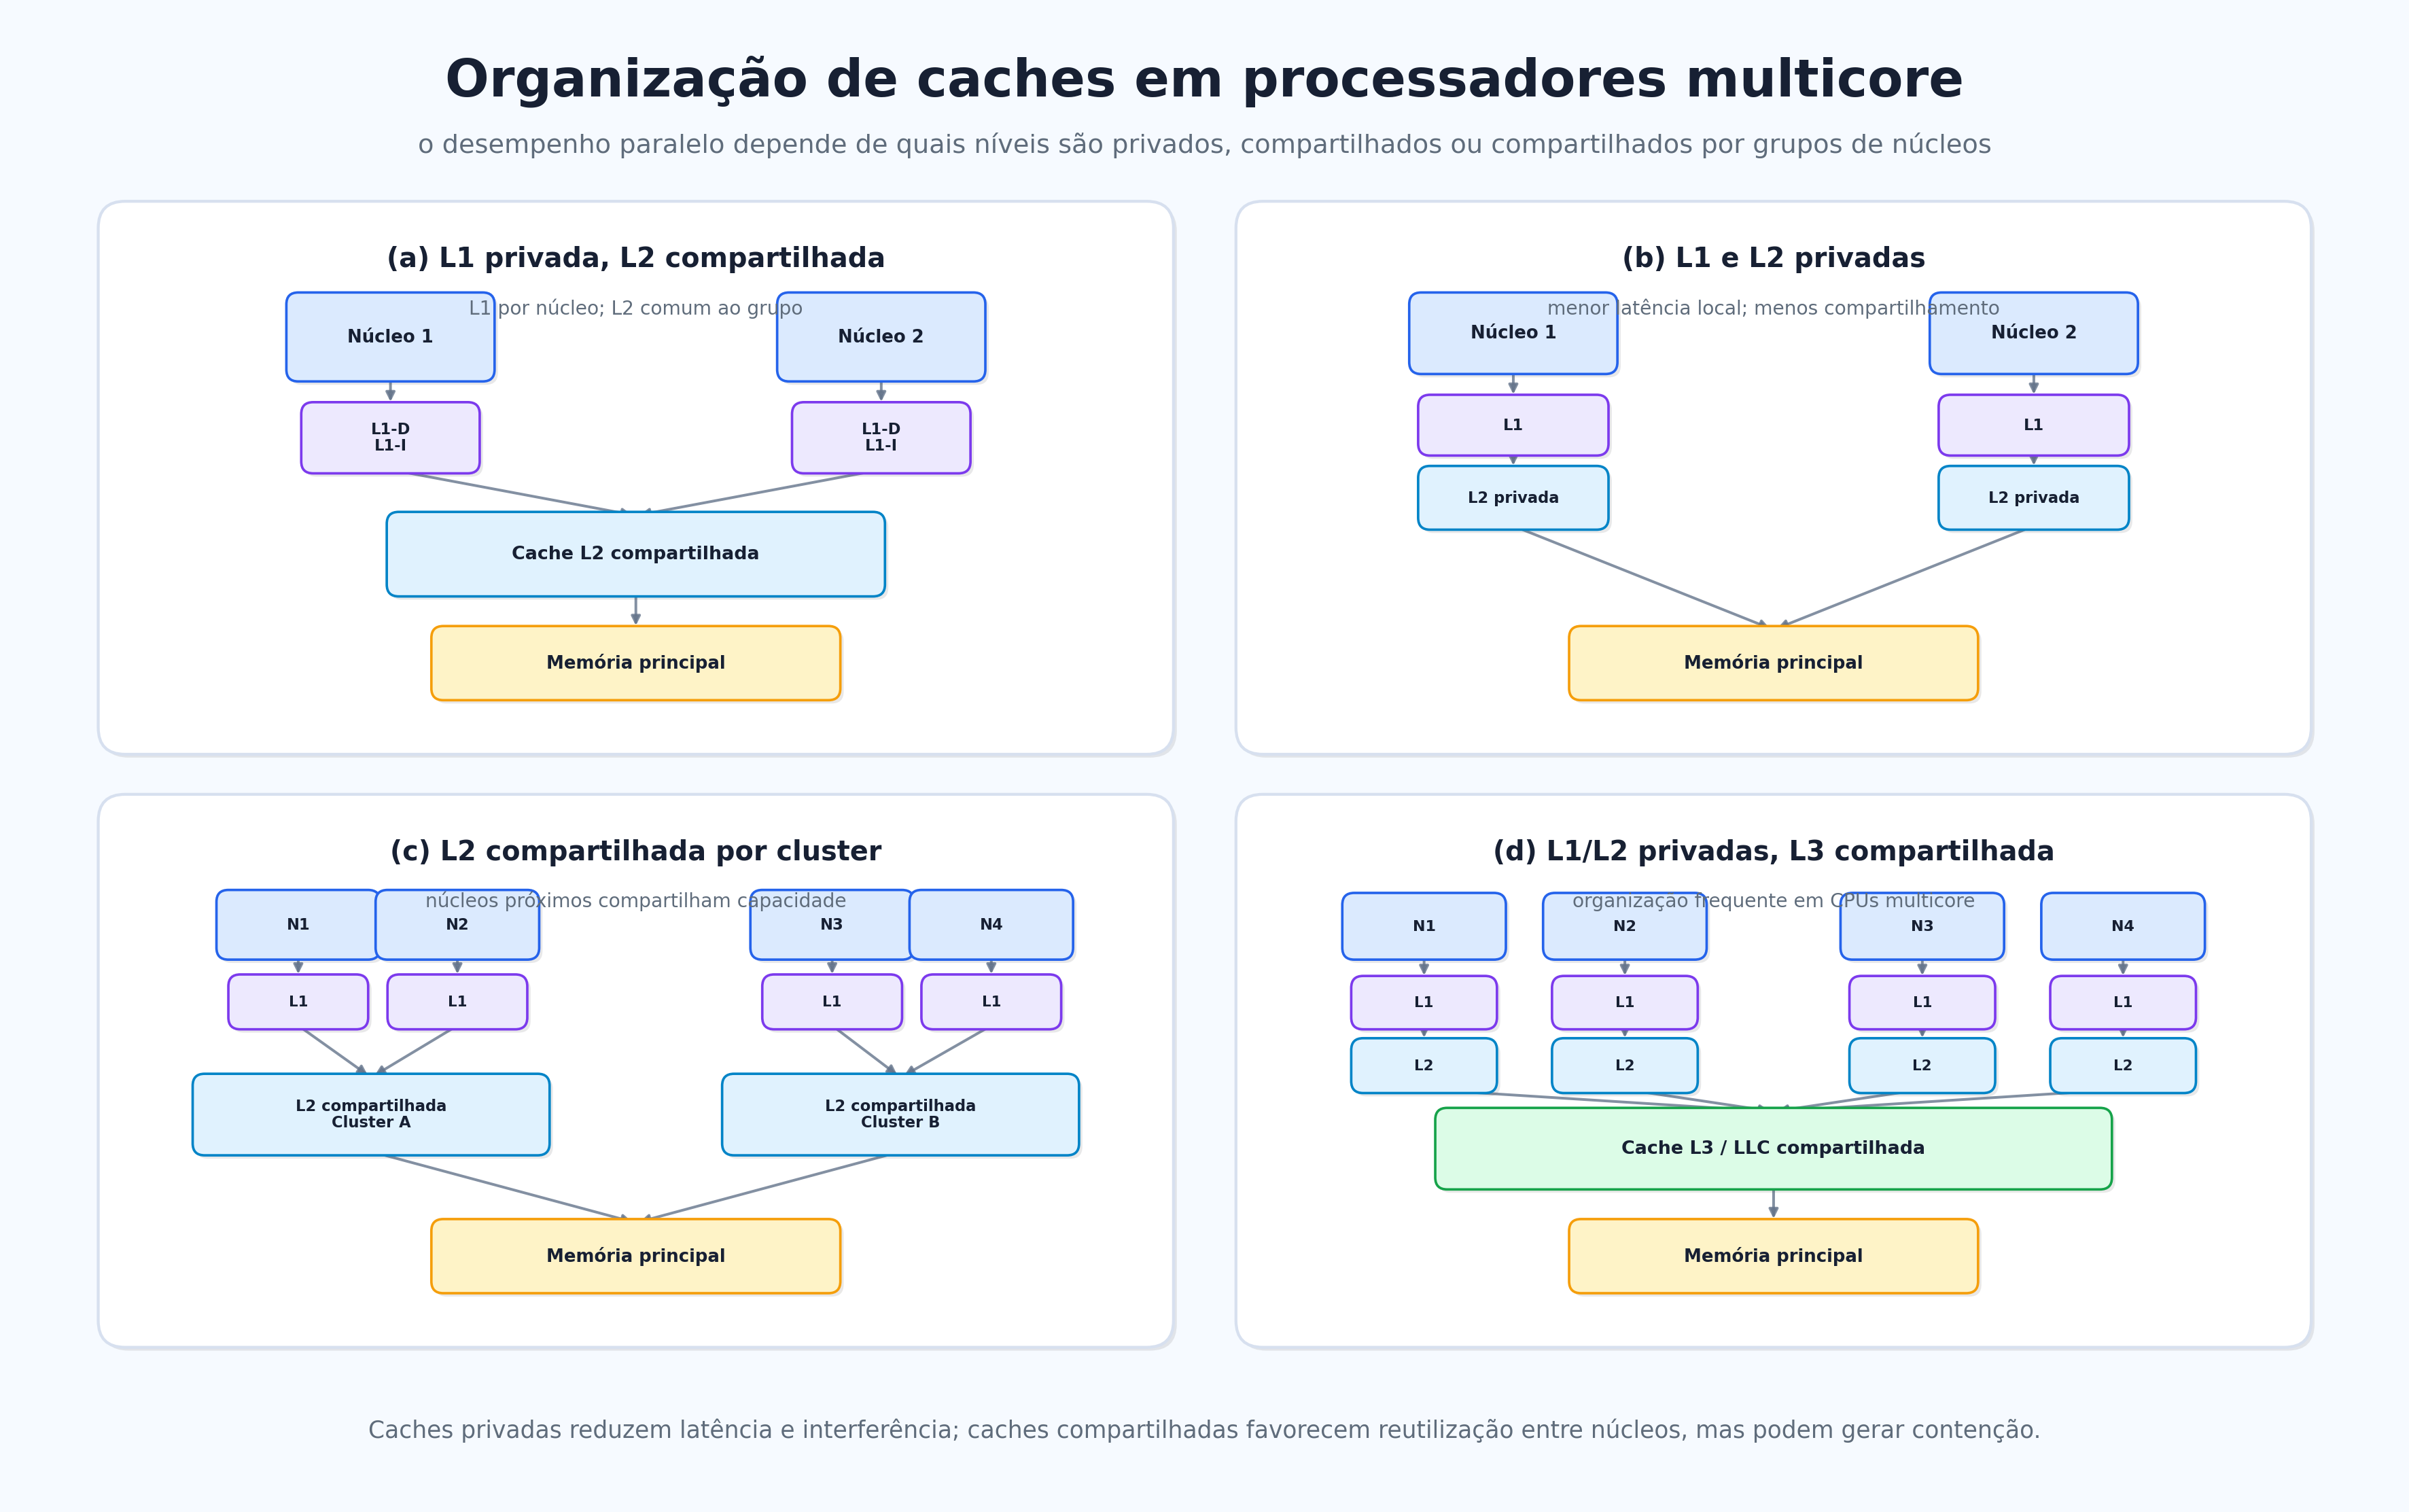
\includegraphics[width=\linewidth,height=.59\textheight,keepaspectratio]{figs/organizacao_caches_multicore.png}
\end{column}
\end{columns}
\pergunta{Mais núcleos significam sempre redução proporcional do tempo de execução?}
\end{frame}

% 04
\begin{frame}{CPU e GPU: prioridades arquiteturais diferentes}
\renewcommand{\arraystretch}{1.34}
\begin{tabular}{p{.22\linewidth}p{.34\linewidth}p{.34\linewidth}}
\toprule
& \textbf{CPU multicore} & \textbf{GPU} \\
\midrule
Prioridade & Latência e flexibilidade & Vazão de operações \\
Paralelismo & Poucas a dezenas de threads de hardware por processador, tipicamente & Grande quantidade de threads CUDA \\
Controle & Forte suporte a fluxos complexos & Melhor aproveitamento de trabalho regular \\
Exemplo & Laços sequenciais, serviços e controle & Muitos elementos de uma matriz \\
\bottomrule
\end{tabular}
\vspace{4mm}
\centering\small A GPU \textbf{não substitui} a CPU: em CUDA, normalmente as duas colaboram.
\end{frame}

% 05
\begin{frame}{Organização conceitual de uma GPU}
\centering
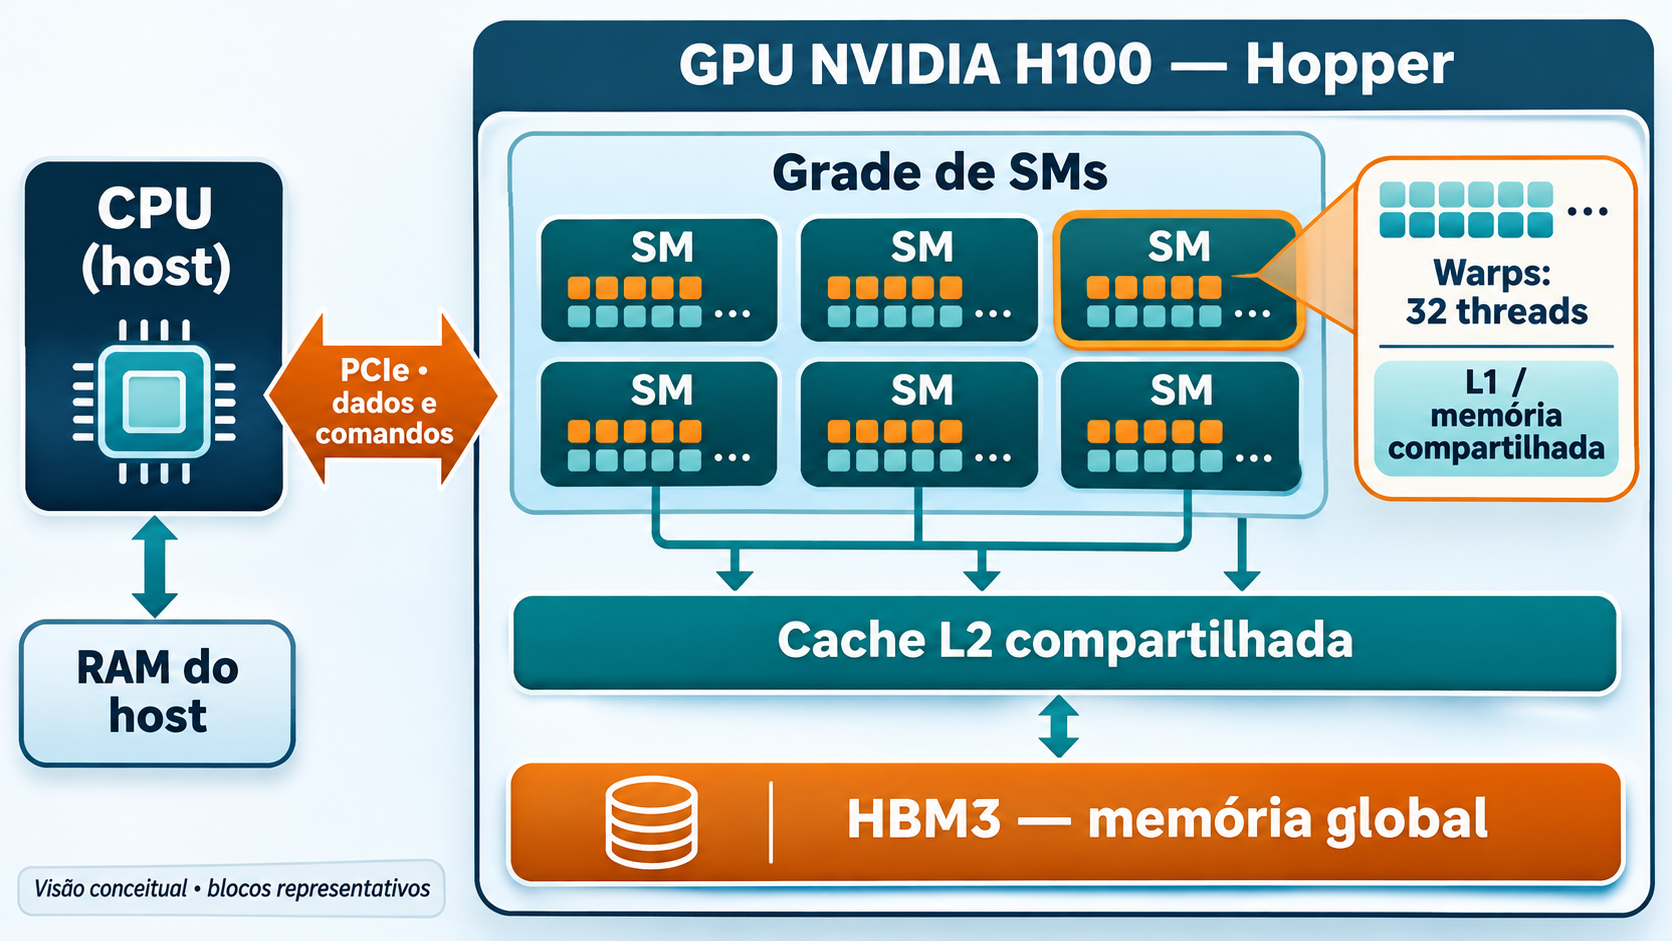
\includegraphics[width=\linewidth,height=.86\textheight,keepaspectratio]{figs/arquitetura_gpu_conceitual.png}
\end{frame}

% 06
\begin{frame}{Três palavras-chave: SM, warp e SIMT}
\begin{description}
\item[SM] \emph{Streaming Multiprocessor}: unidade da GPU que executa e gerencia grupos de threads.
\item[Warp] Grupo de \textbf{32 threads} organizado para execução na arquitetura NVIDIA.
\item[SIMT] \emph{Single Instruction, Multiple Threads}: threads seguem um kernel comum, cada uma com seus próprios dados e índices.
\end{description}
\ideia{A GPU organiza muitos warps em seus SMs; lançar threads não significa executar todas exatamente no mesmo instante.}
\end{frame}

% 07
\begin{frame}{A NVIDIA H100 no Santos Dumont II}
\begin{columns}[T]
\begin{column}{.55\linewidth}
\begin{itemize}
\item GPU NVIDIA \textbf{H100}, geração \textbf{Hopper}.
\item \emph{Compute capability} 9.0: alvo de compilação \texttt{sm\_90}.
\item Neste experimento, solicitaremos \textbf{uma GPU} em um job Slurm.
\item Usaremos CUDA C++ com o compilador \texttt{nvcc}.
\end{itemize}
\end{column}
\begin{column}{.42\linewidth}
\begin{block}{O que NÃO usaremos hoje}
\begin{itemize}
\item Tensor Cores;
\item cuBLAS;
\item \emph{tiling} em memória compartilhada;
\item múltiplas GPUs.
\end{itemize}
\end{block}
\end{column}
\end{columns}
\pergunta{Se a GPU é tão poderosa, por que não devemos esperar uma aceleração enorme para uma matriz 4×4?}
\end{frame}

% 08
\begin{frame}{O problema: multiplicar duas matrizes quadradas}
\centering
\[\boxed{C=A\times B}\qquad C_{ij}=\sum_{k=0}^{N-1} A_{ik}\,B_{kj}\]
\vspace{1mm}
\begin{columns}[T]
\begin{column}{.48\linewidth}
\begin{block}{O que calcular?}
Para calcular \(C_{ij}\):
\begin{enumerate}
\item escolha a \textbf{linha} \(i\) de \(A\);
\item escolha a \textbf{coluna} \(j\) de \(B\);
\item multiplique termos correspondentes e some.
\end{enumerate}
\end{block}
\end{column}
\begin{column}{.48\linewidth}
\begin{exampleblock}{Exemplo com N = 4}
Se \(B\) tem apenas valores 1 e a primeira linha de \(A\) é \((1,2,3,4)\), então
\[C_{0,0}=1+2+3+4=10.\]
O mesmo vale para as outras colunas de \(B\).
\end{exampleblock}
\end{column}
\end{columns}
\end{frame}

% 09
\begin{frame}[fragile]{Versão sequencial: três laços em C}
\begin{lstlisting}[style=prog]
for (int linha = 0; linha < n; linha++) {
    for (int coluna = 0; coluna < n; coluna++) {
        float soma = 0.0f;
        for (int k = 0; k < n; k++) {
            soma += A[linha*n + k] * B[k*n + coluna];
        }
        C[linha*n + coluna] = soma;
    }
}
\end{lstlisting}
\begin{itemize}
\item Os dois primeiros laços percorrem as posições da matriz resultado.
\item O terceiro acumula os produtos necessários para \textbf{uma} posição.
\item Os valores de \(C\) são calculados um após o outro neste código sequencial.
\end{itemize}
\end{frame}

% 10
\begin{frame}{A ideia paralela: uma thread por elemento de C}
\centering
\begin{tikzpicture}[scale=1.0]
  \foreach \i in {0,...,3} {
    \foreach \j in {0,...,3} {
      \pgfmathtruncatemacro{\q}{\i*4+\j}
      \pgfmathsetmacro{\xx}{\j*1.15}
      \pgfmathsetmacro{\yy}{-\i*.82}
      \node[draw=teal,fill=teal!8,minimum width=1.05cm,minimum height=.72cm,inner sep=1pt] at (\xx,\yy) {\small $C_{\i\j}$};
    }
  }
  \node[draw=orange,thick,rounded corners=4pt,inner sep=7pt,fit=(current bounding box)] {};
  \node[font=\small,align=center,anchor=west] at (5.25,-.65) {16 elementos de $C$\\$\Downarrow$\\16 threads CUDA\\\textbf{1 bloco 4$\times$4}};
  \node[font=\scriptsize,align=center] at (1.72,-3.75) {Em cada posição, uma thread faz o laço interno sobre $k$.};
\end{tikzpicture}
\end{frame}

% 11
\begin{frame}[fragile]{Como cada thread descobre a própria posição?}
\begin{lstlisting}[style=prog]
int linha  = blockIdx.y * blockDim.y + threadIdx.y;
int coluna = blockIdx.x * blockDim.x + threadIdx.x;
\end{lstlisting}
\begin{tabular}{p{.24\linewidth}p{.68\linewidth}}
\toprule
\textbf{Identificador} & \textbf{Significado}\\
\midrule
\texttt{threadIdx} & Posição da thread dentro do bloco. \\
\texttt{blockIdx} & Posição do bloco dentro do grid. \\
\texttt{blockDim} & Quantidade de threads em cada dimensão do bloco. \\
\texttt{gridDim} & Quantidade de blocos em cada dimensão do grid. \\
\bottomrule
\end{tabular}
\vspace{3mm}
\pergunta{O que acontece com \texttt{linha} e \texttt{coluna} se a thread está no bloco (1,0), posição local (2,3), com bloco 16$\times$16?}
\end{frame}

% 12
\begin{frame}[fragile]{Kernel CUDA completo (o cálculo na GPU)}
\begin{lstlisting}[style=prog]
__global__ void multiplicar_gpu(
    const float *A, const float *B, float *C, int n) {

    int linha  = blockIdx.y * blockDim.y + threadIdx.y;
    int coluna = blockIdx.x * blockDim.x + threadIdx.x;

    if (linha < n && coluna < n) {
        float soma = 0.0f;
        for (int k = 0; k < n; k++) {
            soma += A[linha*n + k] * B[k*n + coluna];
        }
        C[linha*n + coluna] = soma;
    }
}
\end{lstlisting}
\small \textbf{Nova ideia:} o mesmo código é executado por muitas threads, com diferentes valores de \texttt{linha} e \texttt{coluna}.
\end{frame}

% 13
\begin{frame}{Comparando C e CUDA}
\begin{columns}[T]
\begin{column}{.49\linewidth}
\begin{block}{CPU sequencial}
\begin{itemize}
\item \texttt{for(linha)}
\item \texttt{for(coluna)}
\item \texttt{for(k)}
\item Um fluxo percorre a matriz toda.
\end{itemize}
\end{block}
\end{column}
\begin{column}{.49\linewidth}
\begin{block}{GPU: kernel CUDA}
\begin{itemize}
\item A thread fornece \texttt{linha}.
\item A thread fornece \texttt{coluna}.
\item Cada thread mantém seu \texttt{for(k)}.
\item Muitas posições podem progredir concorrentemente.
\end{itemize}
\end{block}
\end{column}
\end{columns}
\vspace{3mm}
\ideia{O paralelismo está entre os elementos de \(C\), não dentro da soma acumulada por uma thread.}
\end{frame}

% 14
\begin{frame}[fragile]{Bloco e grid: como lançar o kernel}
\begin{lstlisting}[style=prog]
int lado = (n == 4) ? 4 : 16;
dim3 bloco(lado, lado);
dim3 grade((n + lado - 1)/lado, (n + lado - 1)/lado);

multiplicar_gpu<<<grade, bloco>>>(d_A, d_B, d_C, n);
\end{lstlisting}
\begin{itemize}
\item Para \(N=4\): 1 bloco com \(4\times4=16\) threads.
\item Para \(N=512\): \(32\times32=1024\) blocos de \(16\times16=256\) threads.
\item São threads \textbf{lógicas}; a GPU as distribui ao longo do tempo entre seus SMs.
\end{itemize}
\begin{alertblock}{Por que testar os limites?}
O \texttt{if (linha < n \&\& coluna < n)} evita acessar posições fora da matriz em blocos da borda.
\end{alertblock}
\end{frame}

% 15
\begin{frame}[fragile]{Host e device: as duas memórias}
\begin{columns}[T]
\begin{column}{.50\linewidth}
\begin{lstlisting}[style=prog]
cudaMalloc((void**)&d_A, bytes);
cudaMalloc((void**)&d_B, bytes);
cudaMalloc((void**)&d_C, bytes);

cudaMemcpy(d_A, A, bytes,
    cudaMemcpyHostToDevice);
cudaMemcpy(d_B, B, bytes,
    cudaMemcpyHostToDevice);
\end{lstlisting}
\end{column}
\begin{column}{.46\linewidth}
\begin{block}{Quem é quem?}
\begin{itemize}
\item \texttt{A}, \texttt{B}, \texttt{C\_cpu}: memória acessada pela CPU.
\item \texttt{d\_A}, \texttt{d\_B}, \texttt{d\_C}: buffers na GPU.
\item As cópias custam tempo.
\end{itemize}
\end{block}
\end{column}
\end{columns}
\vspace{2mm}
\small \textbf{Depois do kernel:} copiar \texttt{d\_C} da GPU para \texttt{C\_gpu} na CPU, verificar os resultados e liberar a memória.
\end{frame}

% 16
\begin{frame}{Fluxo completo do programa CUDA}
\centering
\begin{tikzpicture}[node distance=3mm,>=Latex,
 box/.style={draw=azul,rounded corners,fill=claro,align=center,minimum width=2.9cm,minimum height=.83cm,font=\small},
 arr/.style={-{Latex[length=2.4mm]},thick,draw=teal}]
\node[box] (n1) {CPU: criar matrizes\\e referência sequencial};
\node[box,right=of n1] (n2) {GPU: alocar buffers\\e copiar $A$, $B$};
\node[box,right=of n2] (n3) {GPU: lançar kernel\\$C=A\times B$};
\node[box,below=1.0cm of n3] (n4) {CPU: receber $C$\\e conferir resultados};
\node[box,left=of n4] (n5) {Medir CPU, kernel\\e transferências};
\draw[arr] (n1)--(n2);\draw[arr] (n2)--(n3);\draw[arr] (n3)--(n4);\draw[arr] (n4)--(n5);
\end{tikzpicture}
\vspace{5mm}
\ideia{A CPU organiza a execução; a GPU realiza o kernel; as transferências fazem parte do custo total da aplicação.}
\end{frame}

% 17
\begin{frame}{Conferência: resultado da multiplicação 4$\times$4}
\centering
\[A=\begin{bmatrix}1&2&3&4\\5&6&7&8\\9&10&11&12\\13&14&15&16\end{bmatrix}
\qquad
B=\begin{bmatrix}1&1&1&1\\1&1&1&1\\1&1&1&1\\1&1&1&1\end{bmatrix}\]
\vspace{-1mm}
\[\boxed{C=\begin{bmatrix}10&10&10&10\\26&26&26&26\\42&42&42&42\\58&58&58&58\end{bmatrix}}\]
\vspace{1mm}
\small \textbf{Primeiro confirme os números!} Medir tempo de um programa incorreto não tem valor.
\end{frame}

% 18
\begin{frame}{Três medidas: o que realmente estamos comparando?}
\renewcommand{\arraystretch}{1.35}
\begin{tabular}{p{.31\linewidth}p{.60\linewidth}}
\toprule
\textbf{Medida} & \textbf{Inclui o quê?}\\
\midrule
CPU sequencial & Apenas o cálculo \(C=A\times B\) na CPU.\\
GPU: kernel & Execução do kernel, medida com eventos CUDA.\\
GPU: transferência + kernel & Copiar \(A\) e \(B\) para a GPU, executar o kernel, copiar \(C\) de volta.\\
\bottomrule
\end{tabular}
\vspace{4mm}
\begin{alertblock}{Comparação justa}
O tempo de \textbf{kernel} isolado não representa o custo total da aplicação GPU. O exemplo não inclui \texttt{cudaMalloc} no tempo total e não é um benchmark otimizado.
\end{alertblock}
\end{frame}

% 19
\begin{frame}[fragile]{Compilar para a NVIDIA H100 (sm\_90)}
\begin{lstlisting}[style=terminal]
module load arch_gpu/current
module load cuda/12.9

cd codigo
make cpu
make gpu
\end{lstlisting}
\begin{itemize}
\item \texttt{nvcc} compila arquivos \texttt{.cu}.
\item \texttt{-arch=sm\_90} seleciona a geração Hopper/H100.
\item \texttt{make cpu} funciona em máquinas sem GPU NVIDIA.
\item \textbf{No SDumont II:} execute o CUDA dentro de um job que aloque GPU.
\end{itemize}
\end{frame}

% 20
\begin{frame}[fragile]{Submeter o experimento no Santos Dumont II}
\begin{lstlisting}[style=terminal]
# Ja dentro da pasta codigo/ no Santos Dumont II
sacctmgr list user "$USER" -s format=partition%20,account
sbatch --account=SEU_PROJETO job_h100.sbatch

# Depois da submissao
squeue -u "$USER"
cat cuda_h100_NUMERO_DO_JOB.out
\end{lstlisting}
\begin{itemize}
\item O script pede 1 GPU e 10 minutos na partição de desenvolvimento indicada.
\item \texttt{SEU\_PROJETO} depende da autorização do usuário no Slurm.
\item O script executa \(N=4,256,512,1024\).
\end{itemize}
\begin{alertblock}{Regra de uso}Não execute kernels ou benchmarks nos nós de login.\end{alertblock}
\end{frame}

% 21
\begin{frame}{Investigação: o que observar?}
\begin{enumerate}
\item \textbf{N=4:} confirme \(C\) e identifique o trabalho de uma thread.
\item \textbf{N=256,512,1024:} anote tempo da CPU, do kernel e do total GPU.
\item Compare os tempos: quando a GPU começa a compensar?
\item Calcule \(S=T_{\mathrm{CPU}}/T_{\mathrm{GPU,total}}\) e discuta o denominador.
\item Explique por que esta versão não explora todos os recursos da H100.
\end{enumerate}
\pergunta{A GPU acelerou o \emph{cálculo} e/ou a \emph{aplicação inteira}? São conclusões diferentes.}
\end{frame}

% 22
\begin{frame}{Fechamento: o que aprendemos?}
\begin{itemize}
\item \textbf{CPU multicore:} vários núcleos executam threads e compartilham recursos de memória.
\item \textbf{GPU:} muitos SMs gerenciam warps de threads em um modelo SIMT.
\item \textbf{CUDA:} cada thread calcula uma posição independente de \(C\).
\item \textbf{Desempenho:} depende do tamanho do problema, da movimentação de dados e do kernel.
\item \textbf{H100:} hardware poderoso; este kernel é \emph{didático}, sem Tensor Cores/cuBLAS.
\end{itemize}
\begin{block}{Próxima questão}
Como reutilizar blocos de \(A\) e \(B\) para reduzir acessos à memória global? (\emph{tiling})
\end{block}
\end{frame}

% 23
\begin{frame}{Referências e materiais de apoio}
\begin{itemize}
\item Slides anteriores: \textbf{Arquiteturas Paralelas e ILP} (disciplina).
\item NVIDIA: \emph{CUDA C++ Programming Guide}.
\item NVIDIA: \emph{Hopper Tuning Guide}; compute capability 9.0.
\item LNCC: \emph{Manual do Supercomputador Santos Dumont II}.
\item Nesta pasta: \texttt{codigo/matriz\_cpu.c}, \texttt{codigo/matriz\_h100.cu}, \texttt{codigo/job\_h100.sbatch}.
\end{itemize}
\vspace{5mm}
\centering\small Os exemplos permitem reproduzir os resultados: nenhuma tabela de tempos foi preenchida antecipadamente.
\end{frame}
\end{document}
